% !TeX root = ../dokumentation.tex

\chapter{Teamorganisation}

\section{Rollenverteilung}
    Zusätzlich zu den klassischen Scrum-Rollen Product-Owner, Scrum-Master und Entwickler 
    wurden im Projekt weitere Rollen eingeführt: Architekten und Service-Leads (vgl. \ref*{fig:Rollenverteilung}). 
    Grundsätzliches Ziel war es die Komplexität des Projektes durch Arbeitsteiltung und feste Ansprechpartner abzufangen.
    Damit sollte auch eine Zusammenarbeit trotz verschiedener Kenntnisstände zu ermöglichen und einen Wissensaustausch zu erleichtern.   

    Die Aufgabe des Produkt-Owners ist es, den Wert des Produkts bzw. des Projekts
    zu maximieren. Mit Hilfe des Backlogs und der Priorisierung der Aufgaben darin stellt der Produkt Owner
    sicher, dass das Team an den richtigen Aufgaben arbeitet.
    Zusätzlich wurden in unserem Team die Storys vom Product Owner erstellt und die Estimation- sowie Planning-Meetings geplant.

    Ein Scrum-Master ist vergleichbar mit einem Teamleiter. Er kümmert sich darum, dass
    das Team (Entwickler und PO) ihrer Arbeit bestmöglich nachgehen können und schützt
    das Team vor ungewolltem Einfluss von außen. Zusammenfassend kann
    man sagen, dass der Scrum-Master dafür verantwortlich ist, dass sich das Team selbst
    organisieren und arbeiten kann. Der Scrum-Master hat auch die Aufgabe, darauf zu achten, dass das Team sich an die
    Scrum-Regeln hält, also alle Meetings regelmäßig durchgeführt werden und tritt wenn nötig in den Meetings als Moderator auf.

    Die Architekten sind für die grundsätzliche Infrastruktur im Projekt zuständig. 
    Dazu entwarfen sie eine Service-übergreifende Architektur und bestimmten nach Evalurierung die eingesetzten Technologien.
    Ziel war es, dass die Architekten einen Gesamtüberblick über das Projekt behalten, 
    und somit Kommunikation zwischen den Services ermöglichen.
     
    
    Service-Leads sind die Ansprechpartner für die einzelnen Services. Dabei sollen sie einen detaillierteren Überblick über die Services behalten 
    und bei Fragen des Teams zur Verfügung stehen. 
    Da die Service-Leads einen besseren Überblick über den Service haben, 
    übernehmen Sie standardmäßig die Reviews von service-spezifischen Tickets und Pull-Requests in den Service-Repositories.

    \begin{figure}[!hbt]
        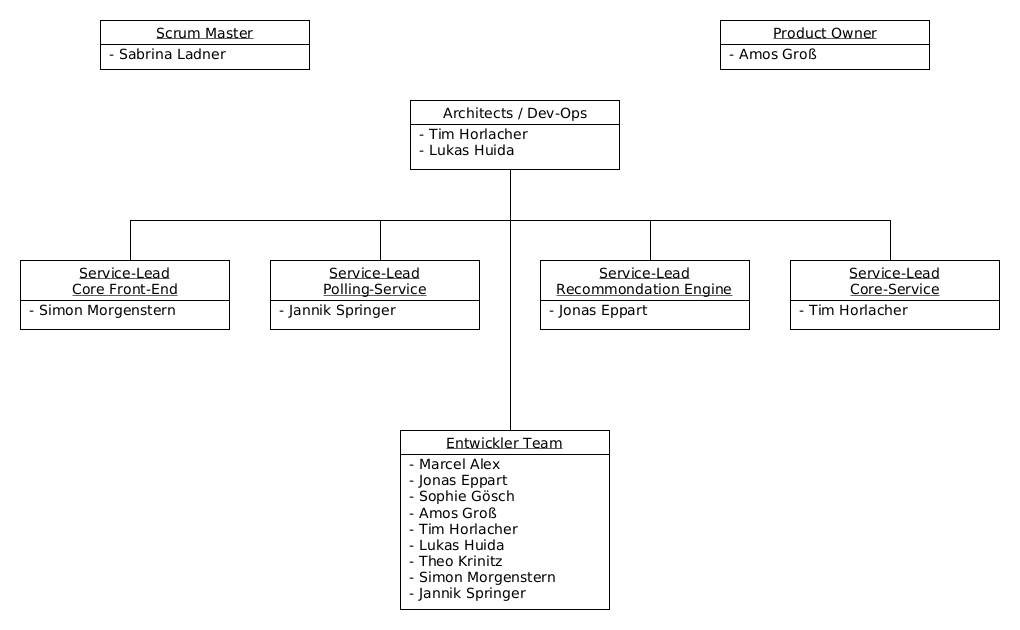
\includegraphics[width=\linewidth]{ProjectOrganigramm2.png}
        \caption{Rollenverteilung}
        \label{fig:Rollenverteilung}
    \end{figure}
    
\section{Eingesetzte Technologien}

\section{Meetings}
Zur Koordination des Teams wurden während des Projektes für Scrum übliche Meetings abgehalten und teilweise an unsere Rahmenbedingungen angepasst.

\subsection{Sprint Planning}
Zu Beginn jedes Sprints findet einmalig das \glqq Sprint Planning\grqq~statt. Dem Namen entsprechend wird in diesem Meeting ein genereller Plan 
für den Sprint erstellt, wofür zuerst vom Product Owner ein Ziel für den Sprint festgelegt wird. Danach werden Tickets aus dem Backlog 
ausgewählt, welche für das Ziel relevant sind und innerhalb des Sprints bearbeitet werden sollen. Dabei wird auch eingeschätzt, wie viel in einem 
Sprint realistisch schaffbar ist. Hierzu werden in \glqq Estimation-Meetings\grqq~die Tickets bezüglich des jeweiligen Arbeitsaufwandes eingeschätzt.
Das Resultat eines \glqq Sprint Plannings\grqq~ist das Sprint-Ziel und der Sprint Backlog.

\subsection{Roadmap-Meeting}
Um im Voraus Storys für das Sprint Planning zu erstellen und auszuplanen erfolgt das \enquote{Roadmap-Meeting}.
Hierbei wurden die Storys, welche vom PO erstellt wurden, mit dem Architekten abgesprochen.
Ziel ist es innerhalb dieses Meetings Storys auf ihre technische Umsetzbarkeit zu kontrollieren und möglicherweise in kleinere aufzuteilen.
Dieses Meeting fand meistens an den Montagen vor den jeweiligen Estimation Meetings statt.

\subsection{Estimation-Meeting}
Innerhalb des \glqq Estimation-Meetings\grqq~werden neue, meist vom Product Owner erstellte Tickets vorgestellt. Nachdem Fragen zum Ticket
geklärt wurden, wird der Arbeitsaufwand des Tickets in Story-Points geschätzt, wobei Fibonacci-Zahlen von 1 bis 21 verwendet werden. Zum Schätzen
gibt jedes Teammitglied eine Zahl an (oder enthält sich) und am Ende wird die Zahl mit den meisten Stimmen übernommen. 
Dieses Meeting findet im Anschluss eines Dailys oder BI-Weeklys statt, wenn seit dem Letzten neue Tickets hinzugefügt wurden.

\subsection{Daily und BI-Weekly}
In \glqq Dailys\grqq~wird von jedem Teammitglied der aktuelle Stand erläutert und Probleme, wie blockierende Tickets oder aufgetretene 
Unklarheiten angesprochen. Normalerweise wird dieses Meeting dem Namen entsprechend täglich abgehalten, ist jedoch in unserem Fall nur einmal 
wöchentlich im Rahmen der Vorlesung vorgesehen. Um einen häufigeren Austausch zu ermöglichen haben wir zusätzlich ein 
\glqq BI-Weekly\grqq~eingeführt, welches inhaltlich dem Daily gleicht und ebenso wöchentlich abgehalten wird.

\subsection{Review}
Zum Abschluss eines Sprints finden \glqq Review\grqq~und danach \glqq Retro\grqq~statt. Im Review wird besprochen, was im Sprint erreicht 
wurde und wie dies den allgemeinen Fortschritt des Projektes beeinflusst. Dabei wird auch besprochen, was als Nächstes zu Erreichen ist. 
Als Resultat dessen, kann der Produkt Backlog beeinflusst werden und Ideen für das Planning des nächsten Sprints gesammelt werden. 

\subsection{Retro}
In der \glqq Sprint-Retrospektive\grqq~oder kurz \glqq Retro\grqq~wird die Zusammenarbeit im Team mithilfe verschiedener Retro-Spiele bewertet. 
Dabei wird besprochen, was gut lief und weitergeführt werden sollte, welche Probleme aufgetreten sind, was im weiteren Verlauf des Projektes 
vermieden werden sollte sowie potenzielle Neuerungen, die eingeführt werden sollten. Dies resultiert in sogenannten Action Items, welche das 
besprochene konkretisieren.

